\documentclass{beamer}

\title{Argumentation among Agents:\\Review and Commentary}
\author{Grigore Costin-Teodor \quad Radu Ștefan-Octavian \\ Vasiliu Florin \quad Vintilă Eduard}
\date{}


\usetheme{Frankfurt}
\setbeamerfont{itemize/enumerate subbody}{size=\normalsize}

\usepackage{tikz}
\usetikzlibrary{arrows.meta}

\newtheorem{Def}{Definition}[subsection]
\newtheorem{Claim}{Claim}

\newcommand{\df}{\ensuremath{\rightharpoonup}}


\begin{document}

\maketitle

% ===================================================================
\section{Florin}

\begin{frame}
\frametitle{Introduction}
\begin{itemize}
\item Reference: Iyad Rahwan's \emph{Argumentation among Agents}, Chapter 5 in \emph{Multiagent Systems}, by G. Weiss. \pause
\item Our contribution: several new examples, and proofs for some merely stated claims. \pause
\item What is the author attempting to formalize? \pause
\item The philosopher's view of argumentation: the giving of claims in favor or against a statement that is open for debate.
\end{itemize}
\end{frame}

\begin{frame}
\frametitle{Prakken's framework, briefly}
\begin{itemize}
\item Idea: generalize common logics by admitting two kinds of inference rules -- \emph{strict} and \emph{defeasible}. \pause
\item An \emph{argumentation system} is a tuple \( (\mathcal{L}, \mathit{cont}, S, D) \). \pause
\item $\mathcal{L}$ is some ``logical language'' (must contain $\neg$). \pause
\item The function \[ \mathit{cont} : \mathcal{L} \rightarrow \mathcal{P(L)} \] generalizes negation. \pause
\item $S, D$ are respectively the sets of strict/defeasible inference rules.
\end{itemize}
\end{frame}

\begin{frame}
\frametitle{Prakken's framework, briefly}
\begin{itemize}
\item How does the $\mathit{cont}$ function generalize negation? \pause
\item If \( \varphi \in \mathit{cont}(\psi) \), then
  \begin{itemize}
  \item[--] if \( \psi \not\in \mathit{cont}(\varphi) \), then $\varphi$ is a \emph{contrary} of $\psi$;
  \item[--] if \( \psi \in \mathit{cont}(\varphi) \), then $\varphi$ and $\psi$ are \emph{contradictory}.
  \end{itemize} \pause
\item It is mandatory that \[ \neg\varphi \in \mathit{cont}(\varphi) \mbox{\quad and\quad } \varphi \in \mathit{cont}(\neg\varphi) \] for any formula $\varphi$.
\end{itemize}
\end{frame}

\begin{frame}
\frametitle{Prakken's framework, briefly}
\begin{itemize}
\item An \emph{argument} from a knowledge base $\mathcal{K}$ is defined similarly to a deduction in propositional logic. (The members of $\mathcal{K}$ play the role of the hypotheses.) \pause
\item Major difference: incorporation of the used inference rules. \pause
\item The complete framework contains a partial order on defeasible rules. Using it, arguments may be compared.
\end{itemize}
\end{frame}

\begin{frame}
\frametitle{Dung's model}
\begin{itemize}
\item Henceforth, an \emph{argumentation framework} will mean a finite directed graph \( (\mathcal{A}, \rightharpoonup) \), whose nodes are called ``arguments''. The adjacency relation is pronounced ``defeats''. \pause
\item Hence, for arguments $p$, $q$,\quad ``$p \rightharpoonup q$'' means ``$p$ defeats $q$''. \pause
\item Note how the structure of arguments is not taken into account anymore. \pause
\item Objective: define an ``acceptable'' argument.
\end{itemize}
\end{frame}

\begin{frame}
\frametitle{Dung's model}
\begin{figure}
\centering
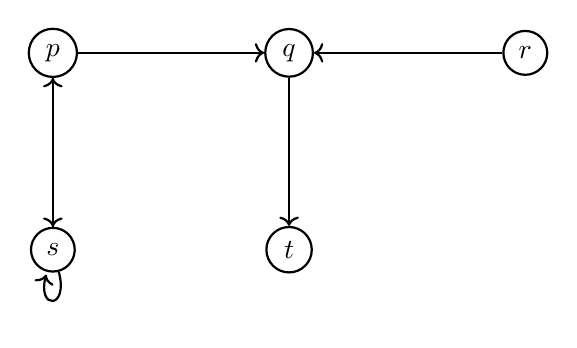
\begin{tikzpicture}
\tikzstyle{vertex} = [circle, draw=black, thick]
\tikzstyle{edge} = [->, thick]
\node[vertex] (p) at (0, 0) {$p$};
\node[vertex] (q) at (3, 0) {$q$};
\node[vertex] (r) at (6, 0) {$r$};
\node[vertex] (s) at (0, -2.5) {$s$};
\node[vertex] (t) at (3, -2.5) {$t$};
\draw[edge] (p)--(q);
\draw[edge] (p)--(s);
\draw[edge] (q)--(t);
\draw[edge] (r)--(q);
\draw[edge] (s)--(p);
\path (s) edge [loop below, thick] node {} (s);
\end{tikzpicture}
\caption{Our argumentation framework.} \label{af}
\end{figure}
\begin{itemize}
\item \( S^{+} = \mbox{ the set of arguments defeated by some member of } S \). \pause
\item In the figure, \( \{ p, q \}^{+} = \{ q, s, t \} \).
\end{itemize}
\end{frame}

\begin{frame}
\frametitle{Dung's model}
\begin{figure}
\centering
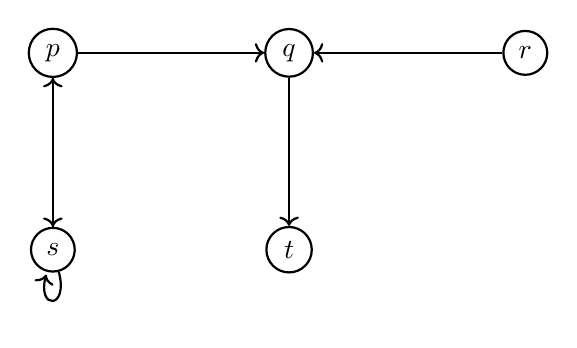
\begin{tikzpicture}
\tikzstyle{vertex} = [circle, draw=black, thick]
\tikzstyle{edge} = [->, thick]
\node[vertex] (p) at (0, 0) {$p$};
\node[vertex] (q) at (3, 0) {$q$};
\node[vertex] (r) at (6, 0) {$r$};
\node[vertex] (s) at (0, -2.5) {$s$};
\node[vertex] (t) at (3, -2.5) {$t$};
\draw[edge] (p)--(q);
\draw[edge] (p)--(s);
\draw[edge] (q)--(t);
\draw[edge] (r)--(q);
\draw[edge] (s)--(p);
\path (s) edge [loop below, thick] node {} (s);
\end{tikzpicture}
\caption{Our argumentation framework.} \label{af}
\end{figure}
\begin{itemize}
\item \( a^{-} = \mbox{ the set of arguments which defeat } a \). \pause
\item In the figure, \( s^{-} = \{ p, s \} \).
\end{itemize}
\end{frame}

\begin{frame}
\frametitle{Dung's model}
\begin{figure}
\centering
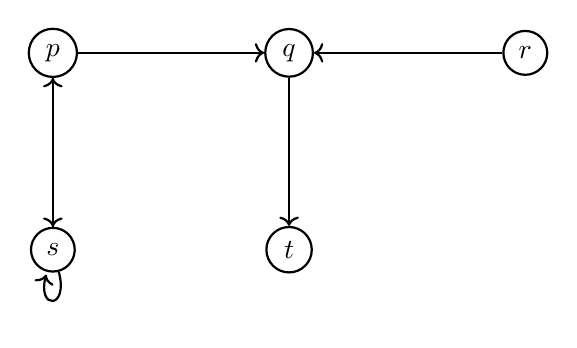
\begin{tikzpicture}
\tikzstyle{vertex} = [circle, draw=black, thick]
\tikzstyle{edge} = [->, thick]
\node[vertex] (p) at (0, 0) {$p$};
\node[vertex] (q) at (3, 0) {$q$};
\node[vertex] (r) at (6, 0) {$r$};
\node[vertex] (s) at (0, -2.5) {$s$};
\node[vertex] (t) at (3, -2.5) {$t$};
\draw[edge] (p)--(q);
\draw[edge] (p)--(s);
\draw[edge] (q)--(t);
\draw[edge] (r)--(q);
\draw[edge] (s)--(p);
\path (s) edge [loop below, thick] node {} (s);
\end{tikzpicture}
\caption{Our argumentation framework.} \label{af}
\end{figure}
\begin{itemize}
\item A set $S$ of arguments is \emph{conflict-free} if no argument in $S$ defeats another also in $S$. \pause
\item In the figure, $\{ p, t \}$ and $\{ r, t \}$ are conflict-free.
\end{itemize}
\end{frame}

\begin{frame}
\frametitle{Dung's model}
\begin{figure}
\centering
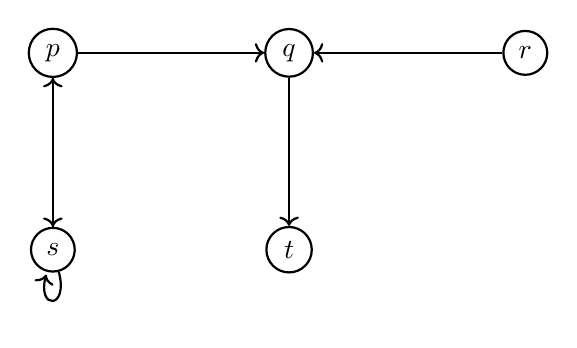
\begin{tikzpicture}
\tikzstyle{vertex} = [circle, draw=black, thick]
\tikzstyle{edge} = [->, thick]
\node[vertex] (p) at (0, 0) {$p$};
\node[vertex] (q) at (3, 0) {$q$};
\node[vertex] (r) at (6, 0) {$r$};
\node[vertex] (s) at (0, -2.5) {$s$};
\node[vertex] (t) at (3, -2.5) {$t$};
\draw[edge] (p)--(q);
\draw[edge] (p)--(s);
\draw[edge] (q)--(t);
\draw[edge] (r)--(q);
\draw[edge] (s)--(p);
\path (s) edge [loop below, thick] node {} (s);
\end{tikzpicture}
\caption{Our argumentation framework.} \label{af}
\end{figure}
\begin{itemize}
\item A set $S$ of arguments \emph{defends} argument $a$ if every argument which defeats $a$ is defeated by $S$ (i.e., is in $S^{+}$). \pause
\item In the figure, $\{ p, t \}$ defends $p$.
\end{itemize}
\end{frame}

\begin{frame}
\frametitle{Dung's model}
\begin{figure}
\centering
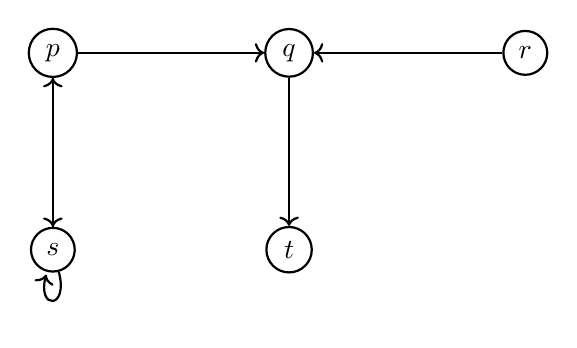
\begin{tikzpicture}
\tikzstyle{vertex} = [circle, draw=black, thick]
\tikzstyle{edge} = [->, thick]
\node[vertex] (p) at (0, 0) {$p$};
\node[vertex] (q) at (3, 0) {$q$};
\node[vertex] (r) at (6, 0) {$r$};
\node[vertex] (s) at (0, -2.5) {$s$};
\node[vertex] (t) at (3, -2.5) {$t$};
\draw[edge] (p)--(q);
\draw[edge] (p)--(s);
\draw[edge] (q)--(t);
\draw[edge] (r)--(q);
\draw[edge] (s)--(p);
\path (s) edge [loop below, thick] node {} (s);
\end{tikzpicture}
\caption{Our argumentation framework.} \label{af}
\end{figure}
\begin{itemize}
\item The \emph{characteristic function} $\mathcal{F}$ is defined thus:\\\centerline{\( \mathcal{F}(S) = \mbox{ the set of arguments defended by } S. \)} \pause
\item In the figure, \( \mathcal{F}(\{ p, q, r \}) = \{ p, r, t \} \) and \( \mathcal{F}(\{ r, t \}) = \{ r, t \} \).
\end{itemize}
\end{frame}

\begin{frame}
\frametitle{Dung's model}
\begin{figure}
\centering
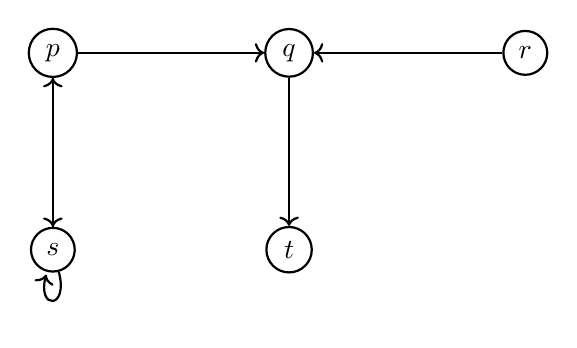
\begin{tikzpicture}
\tikzstyle{vertex} = [circle, draw=black, thick]
\tikzstyle{edge} = [->, thick]
\node[vertex] (p) at (0, 0) {$p$};
\node[vertex] (q) at (3, 0) {$q$};
\node[vertex] (r) at (6, 0) {$r$};
\node[vertex] (s) at (0, -2.5) {$s$};
\node[vertex] (t) at (3, -2.5) {$t$};
\draw[edge] (p)--(q);
\draw[edge] (p)--(s);
\draw[edge] (q)--(t);
\draw[edge] (r)--(q);
\draw[edge] (s)--(p);
\path (s) edge [loop below, thick] node {} (s);
\end{tikzpicture}
\caption{Our argumentation framework.} \label{af}
\end{figure}
\begin{itemize}
\item A \emph{complete extension} is a set $S$ of arguments which is conflict-free and such that \( \mathcal{F}(S) = S \) (i.e., it defends its own members and nothing else). \pause
\item By the remarks on previous slides, $\{ r, t \}$ is a complete extension.
\end{itemize}
\end{frame}

\begin{frame}
\frametitle{Dung's model}
\begin{itemize}
\item The author exhibits an equivalent characterization of complete extensions via \emph{labellings}. \pause
\item An argument $p$ is:
  \begin{itemize}
  \item[--] \emph{skeptically accepted}\quad iff $p$ belongs to every extension;
  \item[--] \emph{credulously accepted}\quad iff $p$ belongs to some extension;
  \item[--] \emph{rejected}\quad iff $p$ doesn't belong to any extension.
  \end{itemize}
\end{itemize}
\end{frame}

% ===================================================================
\section{Eduard}
\begin{frame}
	\frametitle{Argumentation Games}
	\begin{itemize}
		\item The author focuses on Dung's model to present a mechanism by which two agents can participate in a \emph{dispute} where they can state and attack each other's arguments, much as in a real world debate. \pause

		\item Formalize such an argumentation process and additionally enforce a set of constraints in order to capture various semantics (for example, an agent cannot contradict himself).
	\end{itemize}
\end{frame}

\begin{frame}
	\frametitle{Argumentation Games}
	\begin{itemize}
		\item Two players: \textbf{PRO} and \textbf{OPP} \pause

		\item PRO is the proponent which states the initial argument. \pause
		\item OPP is the opponent which begins by counter-attacking the argument proposed by PRO.\pause
		\item Both players take turns in defeating the last argument that has been put forward by their counterpart player.\pause
		\item The game is considered to be won by the player who states an argument $a$ that cannot be defeated (i.e. $a^{-} = \emptyset$)
	\end{itemize}
\end{frame}

\begin{frame}
	\frametitle{What is a dispute?}
	\begin{itemize}
		\item The author calls the sequence of moves done by the players a \emph{dispute}, a notion which is intensively used in further definitions and proofs. \pause
		\item However, a concrete definition is not provided. We attempt to state the following formal definition: \pause
		\begin{Def}[dispute]
			Given an argumentation framework $(\mathcal{A}, \df)$, a dispute is a sequence $(a_{k})_{k \in \mathbb{N}}$ (possibly infinite) of arguments from $\mathcal{A}$ where the following property holds: $\forall i \in \mathbb{N^*},  a_{i} \df a_{i-1}$ (i.e. every argument in the sequence defeats its preceding argument).
		\end{Def}
	\end{itemize}
\end{frame}

\begin{frame}
	\frametitle{Dispute trees}
	\begin{itemize}
		\item Observation: A player could potentially counter-attack its counterpart player with any argument whatsoever that defeats the last move. \pause
		\item This leads to multiple disputes based on the defeating argument chosen by the player, which can be conveniently modeled as a \emph{dispute tree}, as shown by the author.\pause
		\item Again, a definition is not provided. We attempt to adapt one from \emph{Modgil et. al}:\pause
		\begin{Def}[dispute trees]
			Given an argumentation framework\\ $(\mathcal{A}, \df)$ and an argument $p$ in $\mathcal{A}$, a dispute tree induced by $p$ is a tree $T$ rooted in $p$, where each node represents an argument from $\mathcal{A}$ and for all arguments $x, y$ in $\mathcal{A}$, $x$ is a child of $y$ in $T$ iff $x$ defeats $y$.
		\end{Def}
	\end{itemize}
\end{frame}


\begin{frame}
	\frametitle{Protocol $G$}
	\begin{itemize}
		\item The author establishes a rule (called protocol $G$) by which the PRO player cannot repeat an argument in a dispute.\pause
		\item We provide a definition with regards to a decision tree:\pause
		\begin{Def}[dispute tree under protocol G]\label{protG}
			Given a dispute tree $T$, we consider $T$ to be under protocol G iff for any arbitrary dispute $d$ in $T$ and for any pair of arguments $x$, $y$ stated by PRO in $d$, $x$ is different than $y$.
		\end{Def}\pause
		\item It is claimed by the author that the following property is true, to which we provide a proof:\pause

		\begin{Claim}
			If $T$ is a dispute tree under protocol $G$, then $T$ is finite.
		\end{Claim}
	\end{itemize}
\end{frame}

\begin{frame}
	\frametitle{Proof sketch}
	\begin{itemize}
		\item Let $n = card(\mathcal{A})$ and $d = (a_{k})_{k \in \mathbb{N}}$ be a dispute in $T$ of length of at least $2n$ arguments (we do not consider the other disputes, since we know they are of finite length).\pause
		\item We shall prove that $d$ is of finite length; more specifically, exactly of length $2n$. We consider the argument $a_{2n - 1}$ from our sequence $d$.\pause
		\item By protocol G, we have exactly $n$ different arguments uttered by PRO, which cover all the arguments in the set $\mathcal{A}$. \pause
		\item Assume that $a_{2n}$ exists. This being the $n+1$'th argument stated by PRO, it must coincide with an argument that has been uttered before, since we have a total of only $n$ different arguments to choose from (Dirichlet's box principle). \pause
		\item However, this contradicts protocol G. Hence, $d$ is finite.
	\end{itemize}
\end{frame}
% ===================================================================
\section{Ștefan}

% ===================================================================
\section{Costin}
\begin{frame}
\frametitle{The Argument Interchange Format}
\begin{itemize}
\item Stems from a need for standardized representations of arguments. \pause
\item Previous attempts unsuitable: \pause
  \begin{itemize}
  \item[--] designed to be used with specific tools \pause
  \item[--] strong link between language and tool \pause
  \item[--] neglected formal logic due to user experience focus
  \end{itemize}
\end{itemize}
\end{frame}

\begin{frame}
\frametitle{The Argument Interchange Format}
\begin{itemize}
\item Objectives: \pause
  \begin{itemize}
  \item[--] standardize communication between reasoning-based multi-agent systems \pause
  \item[--] facilitate the creation of such systems \pause
  \item[--] design an efficient and abstract format for exchanging data \pause
  \item[--] facilitate argument manipulation and visual representation
  \end{itemize}
\end{itemize}
\end{frame}

\begin{frame}
\frametitle{Foundational concepts of the AIF}
\begin{itemize}
\item Arguments are composed of networks of interlinked nodes. \pause
\item Two types of nodes: \pause
  \begin{itemize}
  \item[--] $\mathcal{N}_I \subset \mathcal{N}$, information nodes (I-nodes) \pause
  \item[--] $\mathcal{N}_S \subset \mathcal{N}$, scheme nodes (S-nodes)
  \end{itemize}
\item Schemes are classes of reasoning patterns. \pause
\item Schemes are divided into: \pause
  \begin{itemize}
  \item[--] $\mathcal{S}^R \subset \mathcal{S}$, \emph{rule of inference} schemes \pause
  \item[--] $\mathcal{S}^C \subset \mathcal{S}$, \emph{conflict} schemes \pause
  \item[--] $\mathcal{S}^P \subset \mathcal{S}$, \emph{preference} schemes
  \end{itemize}
\end{itemize}
\end{frame}

\begin{frame}
\frametitle{Foundational concepts of the AIF}
\begin{itemize}
\item S-nodes are actual \emph{applications} of a scheme. \pause
\item S-nodes are of three types, for each scheme class: \pause
  \begin{itemize}
  \item[--] $\mathcal{N}_S^{RA} \subset \mathcal{N}_S$, rule of inference \emph{application} nodes (\emph{RA-nodes}) \pause
  \item[--] $\mathcal{N}_S^{CA} \subset \mathcal{N}_S$, conflict \emph{application} nodes (\emph{CA-nodes}) \pause
  \item[--] $\mathcal{N}_S^{PA} \subset \mathcal{N}_S$, preference \emph{application} nodes (\emph{PA-nodes}) \pause
  \end{itemize}
\item Example: $MP_1 \in \mathcal{N}_S^{RA}$, an RA-node implementing the modus ponens \emph{rule of inference scheme} from propositional logic.
\end{itemize}
\end{frame}

\begin{frame}
\frametitle{Argument network}
\begin{itemize}
\item An argument network $\Phi$ is a graph, consisting of: \pause
  \begin{itemize}
  \item[--] a set $\mathcal{N} = \mathcal{N}_I \cup \mathcal{N}_S$ of vertices \pause
  \item[--] a binary relation $\xrightarrow{edge}:\mathcal{N}\times\mathcal{N}$, representing edges, with the restriction that $\forall i \in \mathcal{N}_I, \forall j \in \mathcal{N}_I, \not\exists (i,j)\in\xrightarrow{edge}$
  \end{itemize}
\centering
\end{itemize}
\end{frame}

\begin{frame}
\frametitle{A simple argument}
\begin{itemize}
\item A simple argument, in a network $\Phi$ and schemes $\mathcal{S}$ is a tuple $\langle P, \tau, c \rangle$, where: \pause
  \begin{itemize}
  \item[--] $P \subseteq \mathcal{N}_I$ is a set of I-nodes, constituting the premises \pause
  \item[--] $\tau \in \mathcal{N}_S^{RA}$ is an \emph{RA-node} \pause
  \item[--] $c \in \mathcal{N}_I$ is an I-node representing the conclusion, with the condition that $\tau \xrightarrow{edge} c$, uses($\tau, s$), $s \in \mathcal{S}$ and $\forall p \in P$ there is $p \xrightarrow{edge} \tau$
  \end{itemize}
\end{itemize}
\end{frame}


\begin{frame}
\frametitle{Natural language arguments to AIF}
\begin{itemize}
\item The argument: \pause
  \begin{itemize}
  \item[($P_1$)] The sun's UV helps produce Vitamin D in your body \pause
  \item[($P_2$)] Vitamin D is good for your health \pause
  \item[($C_1$)] Therefore, the sun's UV is good for your health \pause
  \end{itemize}
\item We construct the tuple $A_1 = \langle \lbrace P_1, P_2 \rbrace, HS_1, C_1\rangle$, a simple argument in natural language, where $P_1, P_2 \in \mathcal{N}_I$ are premises and $C_1 \in \mathcal{N}_I$ is the conclusion. $HS_1 \in \mathcal{N}_S^{RA}$ is an RA-node, that uses the hypothetical syllogism scheme from propositional logic.
\end{itemize}
\end{frame}


\begin{frame}
\frametitle{Natural language arguments to AIF}
\begin{figure}
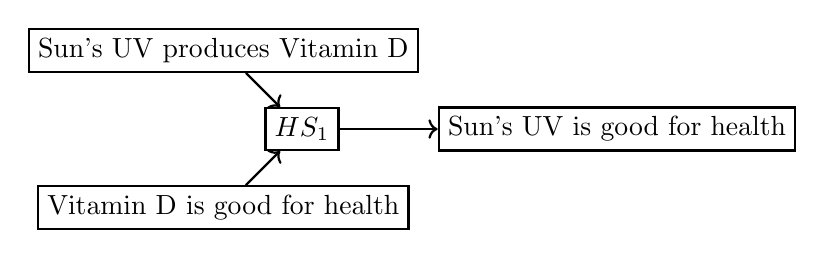
\begin{tikzpicture}
\tikzstyle{vertex} = [rectangle, draw = black, thick]
\tikzstyle{edge} = [->, thick]
\node[vertex] (p) at (0, 0) {Sun's UV produces Vitamin D};
\node[vertex] (HS) at (1, -1) {$HS_1$};
\node[vertex] (q) at (0, -2) {Vitamin D is good for health};
\node[vertex] (r) at (5, -1) {Sun's UV is good for health};
\draw[edge] (p)--(HS);
\draw[edge] (q)--(HS);
\draw[edge] (HS)--(r);
\end{tikzpicture}
\caption{Argument network using natural language} \label{argnet}
\end{figure}
\end{frame}

\begin{frame}
\frametitle{Natural language arguments to AIF}
\begin{itemize}
\item Coming up with a rebuttal: \pause
  \begin{itemize}
  \item[($P_3$)] The sun's UV causes skin cancer \pause
  \item[($P_4$)] Skin cancer is bad for your health \pause
  \item[($C_2$)] Therefore, the sun's UV is bad for your health \pause
  \end{itemize}
\item We use the previous simple argument $A_1 = \langle \lbrace P_1, P_2 \rbrace, HS_1, C_1\rangle$ and similarly define another simple argument $A_2 = \langle \lbrace P_3, P_4 \rbrace, HS_2, C_2\rangle$, where $P_3, P_4 \in \mathcal{N}_I$ are premises and $C_2 \in \mathcal{N}_I$ is the conclusion. $HS_2 \in \mathcal{N}_S^{RA}$ is an RA-node, that uses the hypothetical syllogism scheme from propositional logic. Conflict is displayed with CA-nodes NEG$_1$ and NEG$_2$, instantiations of a conflict scheme based on propositional contraries.
\end{itemize}
\end{frame}

\begin{frame}
\frametitle{Natural language arguments to AIF}
\begin{figure}
\centering
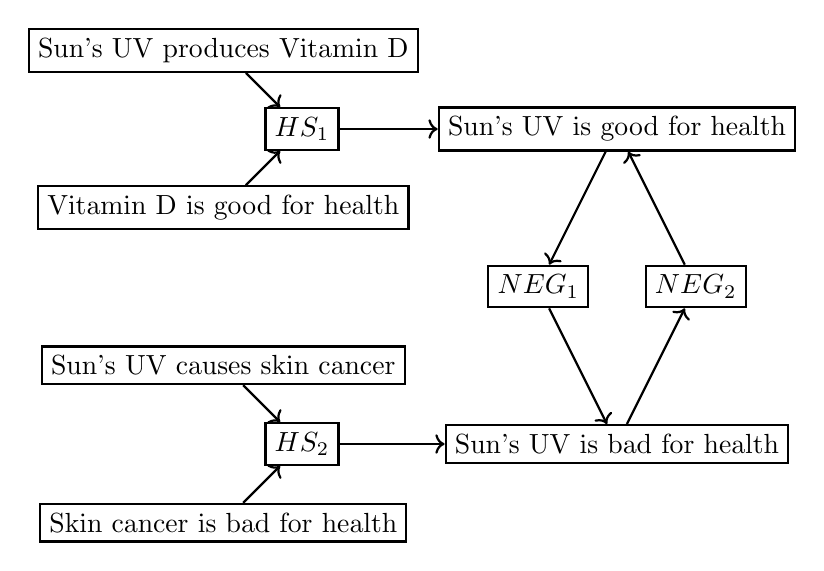
\begin{tikzpicture}
\tikzstyle{vertex} = [rectangle, draw = black, thick]
\tikzstyle{edge} = [->, thick]
% -----------------------------------
% Argument 1
\node[vertex] (p) at (0, 0) {Sun's UV produces Vitamin D};
\node[vertex] (HS1) at (1, -1) {$HS_1$};
\node[vertex] (q) at (0, -2) {Vitamin D is good for health};
\node[vertex] (r) at (5, -1) {Sun's UV is good for health};

\draw[edge] (p)--(HS1);
\draw[edge] (q)--(HS1);
\draw[edge] (HS1)--(r);

% -----------------------------------
% Argument 2
\node[vertex] (x) at (0, -4) {Sun's UV causes skin cancer};
\node[vertex] (HS2) at (1, -5) {$HS_2$};
\node[vertex] (y) at (0, -6) {Skin cancer is bad for health};
\node[vertex] (z) at (5, -5) {Sun's UV is bad for health};

\draw[edge] (x)--(HS2);
\draw[edge] (y)--(HS2);
\draw[edge] (HS2)--(z);
% -----------------------------------
% -----------------------------------
% CA-nodes
\node[vertex] (NEG1) at (4, -3) {$NEG_1$};
\node[vertex] (NEG2) at (6, -3) {$NEG_2$};

\draw[edge] (NEG1)--(z);
\draw[edge] (z)--(NEG2);
\draw[edge] (NEG2)--(r);
\draw[edge] (r)--(NEG1);
% -----------------------------------
\end{tikzpicture}
\caption{Argument network containing a rebuttal in natural language} \label{rebutargnet}
\end{figure}
\end{frame}

% ===================================================================
\end{document}

